\documentclass[crop,tikz]{standalone}
\usetikzlibrary{%
    arrows,
    arrows.meta,
    automata,
    backgrounds,
    calc,
    decorations.pathreplacing,
    fit,
    matrix,
    positioning,
    scopes,
    shadows
}
\usepackage[linguistics]{forest}
\usepackage[charter]{mathdesign}
\tikzset{headarrow/.style = {-{Latex[length=.5em]}}}

\begin{document}
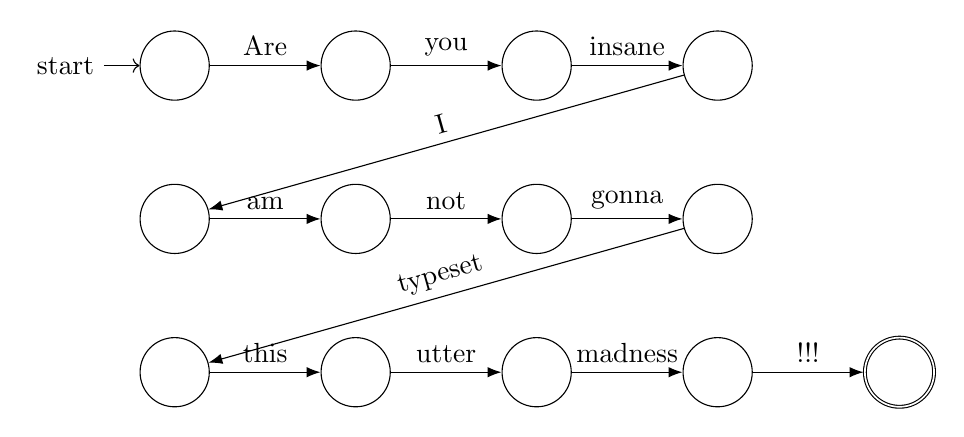
\begin{tikzpicture}
    \node[state,initial] (0-0) at (0,0) {};
    \foreach \x [remember=\x as \lastx (initially 0)] in {1,2,3}
        \node[state] (0-\x) [right=4em of 0-\lastx] {};
    \foreach \x in {0,1,2,3}
        {
        \node[state] (1-\x) [below=3em of 0-\x] {};
        \node[state] (2-\x) [below=3em of 1-\x] {};
        }
    \node[state,accepting] (2-4) [right=4em of 2-3] {};

    \foreach \Source/\Target/\Label in {%
        0-0/0-1/Are,
        0-1/0-2/you,
        0-2/0-3/insane,
        0-3/1-0/I,
        1-0/1-1/am,
        1-1/1-2/not,
        1-2/1-3/gonna,
        1-3/2-0/typeset,
        2-0/2-1/this,
        2-1/2-2/utter,
        2-2/2-3/madness,
        2-3/2-4/!!!}
            \draw[headarrow] (\Source) to node [above,sloped] {\Label} (\Target);
\end{tikzpicture}
\end{document}
